% !TEX program = xelatex
\documentclass[11pt,a4paper]{article}

\usepackage[margin=20mm]{geometry}
\usepackage{fontspec}
\usepackage{microtype}
\usepackage{xcolor}
\usepackage{tikz}
\usepackage{booktabs}
\usepackage{tabularx}
\usepackage{array}
\usepackage{enumitem}
\usepackage{listings}
\usepackage{setspace}
\usepackage{titlesec}
\usepackage{fancyhdr}
\usepackage{graphicx}
\usepackage[most]{tcolorbox}
\usepackage[hidelinks]{hyperref}
\pagecolor{white}

\setmainfont{texgyrepagella-regular.otf}[
  BoldFont = texgyrepagella-bold.otf,
  ItalicFont = texgyrepagella-italic.otf,
  BoldItalicFont = texgyrepagella-bolditalic.otf,
]
\setsansfont{texgyreheros-regular.otf}[
  Scale = 0.94,
  BoldFont = texgyreheros-bold.otf,
  ItalicFont = texgyreheros-italic.otf,
  BoldItalicFont = texgyreheros-bolditalic.otf,
]
\setmonofont{texgyrecursor-regular.otf}[
  Scale = 0.86,
  BoldFont = texgyrecursor-bold.otf,
  ItalicFont = texgyrecursor-italic.otf,
  BoldItalicFont = texgyrecursor-bolditalic.otf,
]

\usetikzlibrary{calc,arrows.meta,positioning}

\definecolor{navy}{HTML}{0F2744}
\definecolor{ice}{HTML}{2E6B8A}
\definecolor{gold}{HTML}{B8893A}
\definecolor{slate}{HTML}{5A6570}
\definecolor{codebg}{HTML}{F4F7F9}
\definecolor{warnbg}{HTML}{FBF4EA}
\definecolor{okbg}{HTML}{EEF6F2}
\definecolor{rule}{HTML}{D5DDE3}

\setstretch{1.12}
\setlist[itemize]{leftmargin=1.15em,itemsep=0.22em,topsep=0.35em}
\setlist[enumerate]{leftmargin=1.3em,itemsep=0.22em,topsep=0.35em}
\setlength{\parindent}{0pt}
\setlength{\parskip}{0.45em}

\titleformat{\section}
  {\sffamily\bfseries\large\color{navy}}
  {\thesection}{0.6em}{}[\vspace{-0.35em}{\color{gold}\titlerule[0.6pt]}\vspace{0.35em}]
\titleformat{\subsection}
  {\sffamily\bfseries\color{ice}}
  {\thesubsection}{0.5em}{}
\titlespacing*{\section}{0pt}{1.15em}{0.45em}
\titlespacing*{\subsection}{0pt}{0.85em}{0.25em}

\pagestyle{fancy}
\fancyhf{}
\renewcommand{\headrulewidth}{0pt}
\fancyhead[L]{\sffamily\footnotesize\color{slate}EnR Guild \textperiodcentered{} IIT Madras}
\fancyhead[R]{\sffamily\footnotesize\color{slate}Hockey RL Competition}
\fancyfoot[C]{\sffamily\footnotesize\color{slate}\thepage}
\fancypagestyle{plain}{\fancyhf{}\renewcommand{\headrulewidth}{0pt}}

\lstdefinestyle{py}{
  language=Python,
  basicstyle=\ttfamily\footnotesize,
  keywordstyle=\bfseries\color{navy},
  commentstyle=\itshape\color{slate},
  stringstyle=\color{ice},
  breaklines=true,
  frame=none,
  backgroundcolor=\color{codebg},
  columns=fullflexible,
  keepspaces=true,
  showstringspaces=false,
  aboveskip=0.55em,
  belowskip=0.55em,
  xleftmargin=0.7em,
  xrightmargin=0.7em,
  framexleftmargin=0.4em,
  morekeywords={self,np},
}
\lstset{style=py}

\tcbset{
  enhanced,
  boxrule=0.7pt,
  arc=1.5pt,
  left=9pt,right=9pt,top=7pt,bottom=7pt,
  fonttitle=\sffamily\bfseries\small,
  coltitle=navy,
}

\newtcolorbox{callout}[1][]{
  colback=okbg, colframe=ice,
  title={#1},
}
\newtcolorbox{warnbox}[1][]{
  colback=warnbg, colframe=gold,
  title={#1},
}

\newcommand{\mono}[1]{\texttt{\detokenize{#1}}}

\begin{document}
\thispagestyle{empty}

% ----- banner -----
\noindent
\begin{tikzpicture}[remember picture, overlay]
  \fill[navy] ([yshift=0mm]current page.north west) rectangle
              ([yshift=-38mm]current page.north east);
  \fill[gold] ([yshift=-38mm]current page.north west) rectangle
              ([yshift=-40mm]current page.north east);
\end{tikzpicture}

\vspace*{-6mm}
{\sffamily\color{white}
{\Large\bfseries EnR Guild}\\[0.15em]
{\LARGE\bfseries Hockey RL Competition}\\[0.35em]
{\large Getting started}
\par}
\vspace{3mm}
{\sffamily\small\color{navy} A recruitment filter, not a Kaggle board. Beat the weak bot, survive the round-robin, then explain what you built.\par}

\vspace{2mm}

\begin{callout}[Do this in the next fifteen minutes]
\begin{enumerate}[leftmargin=1.4em,itemsep=0.15em]
  \item Clone the repo. Use \textbf{Python 3.10--3.12}.
  \item \texttt{python3.12 -m venv .venv \&\& source .venv/bin/activate}
  \item \texttt{pip install -r requirements.txt}\\
        On macOS, if \texttt{box2d-py} fails to build: \texttt{brew install swig} and retry.
  \item \texttt{python submission\_template/agent.py} --- should print \texttt{action shape: (4,)}
  \item \texttt{python scripts/validate\_submission.py submission\_template}
\end{enumerate}
Copy \texttt{submission\_template/} to your working folder. The random policy is a load check, not a competitor.
\end{callout}

\section{What this is}

You train a reinforcement-learning agent to play a two-player, continuous-control hockey game built on Box2D (\href{https://github.com/martius-lab/hockey-env}{martius-lab/hockey-env}). You submit a small folder. We run your agent in isolation against baselines, then against everyone else.

Leaderboard rank is the \emph{entry ticket}. The actual recruitment filter is a short viva with the people who wrote agents that survived Phase~2. We will ask why you chose the algorithm, how you shaped the reward, and what broke.

\section{How you are judged}

\begin{center}
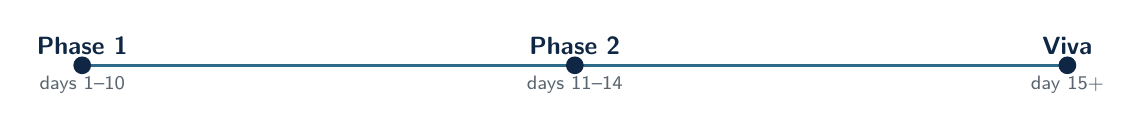
\begin{tikzpicture}[x=18.4mm, y=1]
  \draw[ice, line width=1.15pt] (0,0) -- (6.8,0);
  \foreach \x/\lab/\sub in {
    0/{Phase 1}/{days 1--10},
    3.4/{Phase 2}/{days 11--14},
    6.8/{Viva}/{day 15+}
  } {
    \fill[navy] (\x,0) circle (3.2pt);
    \node[font=\sffamily\bfseries\small, navy, anchor=south] at (\x,0.48) {\lab};
    \node[font=\sffamily\scriptsize, slate, anchor=north] at (\x,-0.42) {\sub};
  }
\end{tikzpicture}
\end{center}

\vspace{0.4em}
\begin{tabularx}{\textwidth}{@{}>{\sffamily\bfseries\color{navy}}p{2.4cm} X@{}}
Phase 1 & Your agent plays \texttt{weak\_bot} and \texttt{strong\_bot} only. Scores are public. Beating the weak bot is the first real signal; a 30--70 loss to the strong bot is still respectable. The public board is not the final ranking. \\[0.45em]
Phase 2 & Standings are wiped. Every valid submission plays every other. Ranking is by \textbf{Elo} (start 1000, $K=32$), not raw win rate. Agents that only memorised the weak bot usually collapse here. \\[0.45em]
Viva & Top 5--8 teams, about ten minutes. Reward design, failure modes, algorithm choice. If you cannot explain a curve in your writeup, the rank will not save you. \\
\end{tabularx}

\section{The contract}

Every submission is a Python file named \texttt{agent.py} that defines exactly this class. \texttt{\_\_init\_\_} loads weights. \texttt{act} is called every physics step. Do not train in \texttt{\_\_init\_\_}.

\noindent\begin{minipage}{\textwidth}
\begin{lstlisting}
class Agent:
    def __init__(self):
        # Load weights. Keep this fast.
        pass

    def act(self, observation: np.ndarray) -> np.ndarray:
        # observation: shape (18,)
        # return:      shape (4,), values in [-1, 1]
        raise NotImplementedError
\end{lstlisting}
\end{minipage}

Eval instantiates \texttt{Agent} once per match process, then calls \texttt{act} thousands of times. A single call that exceeds \textbf{100\,ms} fails validation. Exceptions in \texttt{act} are a forfeit for that episode.

\subsection{Observation --- 18 floats, player-first}

The vector is what \texttt{HockeyEnv} actually returns. Index 0 is \emph{you} when you are player~1. When you are player~2, eval feeds the \emph{mirrored} vector from \texttt{env.obs\_agent\_two()} so you still look like player~1. If you self-play, you must do the same.

\begin{center}
\small
\begin{tabular}{@{}cl l@{}}
\toprule
\sffamily\bfseries Index & \sffamily\bfseries Slice & \sffamily\bfseries Meaning \\
\midrule
0--1  & \texttt{[0:2]}   & Player 1 position $(x,y)$ \\
2     & \texttt{[2]}     & Player 1 angle \\
3--4  & \texttt{[3:5]}   & Player 1 velocity $(v_x,v_y)$ \\
5     & \texttt{[5]}     & Player 1 angular velocity \\
6--7  & \texttt{[6:8]}   & Player 2 position $(x,y)$ \\
8     & \texttt{[8]}     & Player 2 angle \\
9--10 & \texttt{[9:11]}  & Player 2 velocity \\
11    & \texttt{[11]}    & Player 2 angular velocity \\
12--13& \texttt{[12:14]} & Puck position $(x,y)$ \\
14--15& \texttt{[14:16]} & Puck velocity \\
16    & \texttt{[16]}    & Player 1 has-puck timer \\
17    & \texttt{[17]}    & Player 2 has-puck timer \\
\bottomrule
\end{tabular}
\end{center}

\subsection{Action --- 4 floats, clipped to [-1, 1]}

\begin{center}
\begin{tabular}{@{}cl p{9.2cm}@{}}
\toprule
\sffamily\bfseries $i$ & \sffamily\bfseries Control & \sffamily\bfseries Notes \\
\midrule
0 & Force $x$ & Along the length of the rink \\
1 & Force $y$ & Lateral \\
2 & Torque    & Rotation of the mallet \\
3 & Shoot     & Fires when the value is $> 0.5$ \\
\bottomrule
\end{tabular}
\end{center}

Clip before you return. Unclipped actions make Box2D behave oddly. A NORMAL episode is \textbf{250} steps; treat both \texttt{terminated} and \texttt{truncated} as ``game over''.

\begin{center}
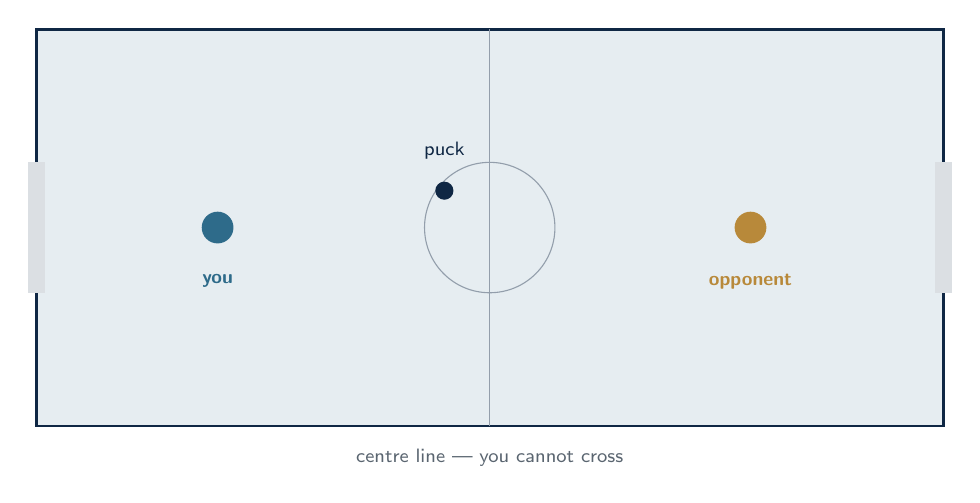
\begin{tikzpicture}[x=7.2mm,y=7.2mm]
  \fill[ice!12] (0,0) rectangle (16,7);
  \draw[navy, line width=1.05pt] (0,0) rectangle (16,7);
  \draw[navy!45] (8,0) -- (8,7);
  \draw[navy!45] (8,3.5) circle (1.15);
  \fill[navy!15] (-0.15,2.35) rectangle (0.15,4.65);
  \fill[navy!15] (15.85,2.35) rectangle (16.15,4.65);
  \fill[ice] (3.2,3.5) circle (0.28);
  \fill[gold] (12.6,3.5) circle (0.28);
  \fill[navy] (7.2,4.15) circle (0.16);
  \node[font=\sffamily\scriptsize\bfseries, ice] at (3.2,2.55) {you};
  \node[font=\sffamily\scriptsize\bfseries, gold] at (12.6,2.55) {opponent};
  \node[font=\sffamily\scriptsize, navy] at (7.2,4.85) {puck};
  \node[font=\sffamily\scriptsize, slate] at (8,-0.55) {centre line --- you cannot cross};
\end{tikzpicture}
\end{center}

\section{Training}

\texttt{submission\_template/train.py} fits Stable-Baselines3 SAC against the built-in \emph{weak} opponent for 500k steps, using \texttt{HockeySingleAgentEnv}. That wrapper steps the opponent internally so SB3 sees a single-agent \texttt{gymnasium} env.

\begin{lstlisting}
python submission_template/train.py --timesteps 500000 --output my_agent
\end{lstlisting}

This is a \textbf{pipeline proof}, not a good agent. Things that actually move the needle: reward shaping (closeness to puck, shot timing, not spinning), a curriculum (weak $\to$ strong $\to$ self-play), longer training, and not overfitting Phase~1.

Load the zip next to \texttt{agent.py}:

\begin{lstlisting}
from stable_baselines3 import SAC

class Agent:
    def __init__(self):
        self.model = SAC.load("my_agent.zip")

    def act(self, observation):
        action, _ = self.model.predict(observation, deterministic=True)
        return np.asarray(action, dtype=np.float32)
\end{lstlisting}

\section{What to submit}

A folder (zip or git link --- we will tell you which) containing:

\begin{center}
\begin{tabular}{@{}ll l@{}}
\toprule
\sffamily\bfseries File & \sffamily\bfseries Required & \sffamily\bfseries \\
\midrule
\texttt{agent.py}         & yes & The class above \\
model weights             & yes & Whatever \texttt{\_\_init\_\_} loads \\
\texttt{requirements.txt} & yes & Extra pip deps, pinned if it matters \\
\texttt{writeup.md}       & \textbf{yes} & See below. No writeup $=$ disqualified \\
\bottomrule
\end{tabular}
\end{center}

A template lives in \texttt{submission\_template/writeup.md}. Four sections, all mandatory:

\begin{enumerate}
  \item \textbf{Algorithm} --- what you trained and why it fits this game.
  \item \textbf{Reward} --- the terms you used and the behaviour each one was for.
  \item \textbf{Something that broke} --- one failure, the evidence, the fix.
  \item \textbf{Training curves} --- labelled plots, not a screenshot of a terminal.
\end{enumerate}

Check locally before you send it:

\begin{lstlisting}
python scripts/validate_submission.py path/to/your_folder
\end{lstlisting}

Exit code 0 means the file loads, \texttt{act} returns shape \texttt{(4,)}, and inference stays under 100\,ms. It does \emph{not} mean the writeup is good.

\section{How evaluation works}

\begin{itemize}
  \item Each match is 20 episodes (unless we say otherwise), sides swapped every episode so you are not stuck on the left.
  \item Player 2 always receives \texttt{obs\_agent\_two()}. You never see the raw player-1 vector when you are on the right.
  \item The match runs in a \textbf{subprocess}. A hang is killed; unfinished episodes count as draws and the match is marked \texttt{timeout}.
  \item Default wall-clock budget is 120 seconds per match. Keep \texttt{act} cheap.
  \item Elo starts at 1000 for every agent, including the built-in bots. The leaderboard sorts by Elo.
\end{itemize}

\begin{warnbox}[Five ways to silently lose]
\begin{enumerate}[leftmargin=1.2em]
  \item Feeding player~2 the raw observation instead of the mirrored one (in your own self-play).
  \item Returning an action that is not shape \texttt{(4,)} or contains NaNs.
  \item Training inside \texttt{Agent.\_\_init\_\_} --- it will time out before the first face-off.
  \item Ignoring \texttt{truncated}. Time-expired games are draws, not wins.
  \item A 200\,ms policy network. Validation will reject you; eval would too.
\end{enumerate}
\end{warnbox}

\section{What ``good'' looks like}

A submission we take seriously usually:

\begin{itemize}
  \item Beats \texttt{weak\_bot} consistently.
  \item Has \emph{some} plan against \texttt{strong\_bot} --- losing 30--70 is fine; spinning in place is not.
  \item Does not degenerate (never moving, always shooting, orbiting its own goal).
  \item Comes with a writeup that could be read aloud in the viva without embarrassment.
\end{itemize}

If the SAC template already ``kind of works,'' that is the starting line. Self-play, opponent sampling, and a reward you can defend are the actual contest.

\vspace{1.1em}
{\sffamily\small\color{slate}Questions go to the EnR Guild organisers. Rebuild this PDF with \texttt{make -C guide pdf}.\par}

\end{document}
